\documentclass[12pt, aspectratio=43]{beamer} 

% 自訂字體的封包
\usepackage{fontspec} 

%% 設定中文字體
\usepackage{xeCJK}
    \setCJKmainfont[AutoFakeBold=3]{SimSun}
    \XeTeXlinebreaklocale "zh"             
    \XeTeXlinebreakskip = 0pt plus 1pt

% 數學工具及符號
\usepackage{mathtools, amsmath, amsfonts, amsthm, amssymb, latexsym} 
\usepackage{relsize}
% background
\usetheme{Darmstadt}
\setbeamertemplate{footline}[page number]{}

% Headers and footers
\usepackage{fancyhdr}

% Inserting Images
\usepackage{graphicx}
\usepackage{subcaption}
\usepackage{float}


% Using colours in LaTeX
\usepackage{color}
\usepackage{multirow}

% Biblatex citation styles
\usepackage[style=numeric,backend=bibtex,sorting=none]{biblatex} 
\bibliography{reference}

% Misc
\usepackage{lipsum}
\usepackage{wrapfig}
\usepackage[document]{ragged2e}
\usepackage{tabularx}
\usepackage{tikz}

\usepackage{hyperref}

\setbeamertemplate{caption}[numbered]
 % 載入封包與文檔配置

% Title, Subtitle, Author, Institute, Date
\title[\textbf{Week 3 Report}]{Week 3 Report}
\author[Chen, Pin-Jui]{Chen, Pin-Jui}
\date[Sep 26, 2025]{Sep 26, 2025}

\begin{document}

% Title page frame
\begin{frame}
  \titlepage
\end{frame}

% Index
\begin{frame}
  \frametitle{Index}
  \tableofcontents
\end{frame}

\section{探討RNA甲基轉移酶NSUN2基金多型性與子宮內膜癌其臨床特徵之影響}
\begin{frame}{What is NSUN2}
    \begin{figure}[h!]
        \centering
        \begin{minipage}{0.6\textwidth}
            \begin{itemize}
                \item \textbf{NSUN2} is a gene.
                \item The gene is transcribed into mRNA, which is then translated into \textbf{NSUN2 protein}.
                \item The \textbf{NSUN2 protein} belongs to the RNA methyltransferase family, which adds $m^5C$ (5-甲基胞嘧啶) modifications to tRNA and mRNA, helping RNA stability and regulating gene expression.
            \end{itemize}
        \end{minipage}\hfill
        \begin{minipage}{0.35\textwidth}
            \centering
            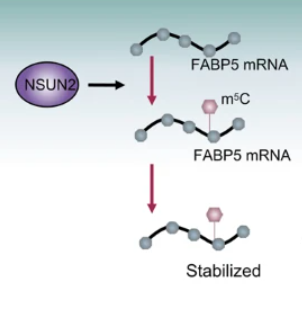
\includegraphics[width=\linewidth]{Figure/NSUN2.png}
            \caption[NSUN2 mechanism]{Illustration of NSUN2 mechanism\cite{Yang2023}}
        \end{minipage}
    \end{figure}
\end{frame}

\begin{frame}{NSUN2 and Cancer}

\begin{itemize}
    \item Cancer cells:
    \begin{itemize}
        \item NSUN2 overexpressed \cite{Okamoto2012}.
        \item Stabilizes oncogenic mRNAs like
	\begin{itemize}
		\item Lung Adenocarcinoma \cite{Li2025}
		\item Pancreatic Cancer \cite{Zhang2023}
		\item Uterine Corpus Endometrial Carcinoma \cite{YangRNA}
	\end{itemize}
        \item Promotes proliferation(增生), metastasis(轉移), and chemoresistance(化療抗藥性)
    \end{itemize}
\end{itemize}
\end{frame}

\begin{frame}{NSUN2 Gene Polymorphisms}
	\begin{itemize}
		\item SNP, Single Nucleotide Polymorphism (單一核苷酸多型性)
		\begin{itemize}
			\item A single-base change in DNA sequence (e.g., C/T, A/G).  
			\item May influence gene expression or protein function. 
		\end{itemize}
		
		\item In this plan, we will examine four key NSUN2 SNPs:
		\begin{itemize}
			\item rs4702373 (C/T)  
			\item rs166049 (T/G)  
			\item rs13181449 (C/T)  
			\item rs8192120 (C/A)
		\end{itemize}
		Some studies have shown that NSUN2 rs13181449 C>T is associated with a reduced risk of cancer, including oral cavity squamous cell carcinoma \cite{Hung2025NSUN2} and neuroblastoma \cite{LIN2023147120}.
	\end{itemize}
\end{frame}

\begin{frame}{Statistical Methods}
	Relationship between cancer stage and NSUN2 SNPs
	
	\begin{itemize}
		\item Determine if SNPs are related to cancer stage
		\begin{itemize}
			\item T-test (for continuous covariates)
			\item Chi-squared test (for categorical variables)
		\end{itemize}
		
		\item Assess the independent effect of SNPs
		\begin{itemize}
			\item Multiple unconditional logistic regression model
			\item Adjusted Odds Ratio (AOR) with 95\% confidence interval
		\end{itemize}
	\end{itemize}
\end{frame}



\section{Single-cell RNA sequencing technologies}
\begin{frame}{scRNA-seq}
	The procedures of scRNA-seq mainly include \cite{jovic2022single} 
	\begin{enumerate}
		\item Single-cell isolation and capture
		\item Cell lysis
		\item Reverse transcription (conversion of their RNA into cDNA)
		\item cDNA amplification
		\item Library preparation
	\end{enumerate}
\end{frame}

\subsection{Single-cell analysis}
\begin{frame}{Single cell RNA Analysis Method}
	\begin{figure}[h!]
		\centering
		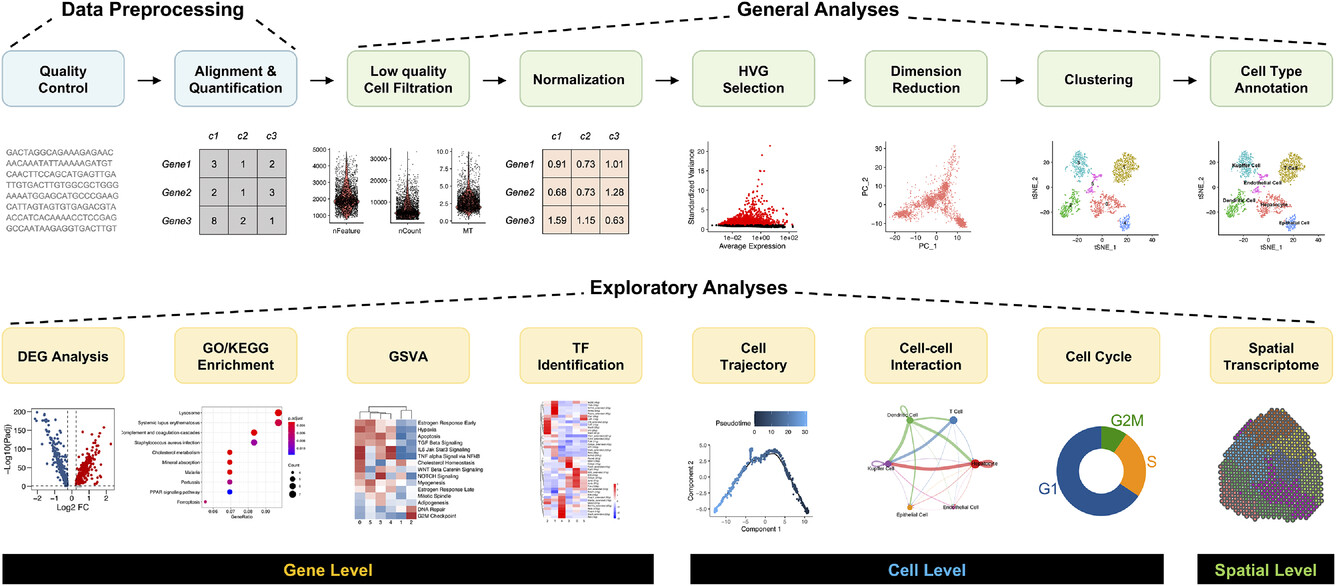
\includegraphics[width=\linewidth]{Figure/analysis.png}
	\end{figure}
\end{frame}

\begin{frame}{Single cell RNA Analysis}
	\begin{itemize}
		\item The single-cell RNA sequencing data set is high-dimensional.
		\item Most genes in each cell belong to housekeeping ones, as they are characterized by \textbf{no significant changes} in the expression level between cells, and their presence tends to obscure the real biological signals.
		\item  The subsets of features that exhibit high cell-to-cell variation in the data set are also called \textbf{highly variable genes (HVGs)}.
		\item A high-quality HVGs should include genes that can distinguish different cell types, and the quality of HVGs has a significant effect on the precision of clustering.
	\end{itemize}
\end{frame}

\begin{frame}{Single cell RNA Analysis}
	\begin{itemize}
		\item \textbf{Batch-effect correction} : \textbf{deepMNN} achieves higher accuracy than commonly used methods, particularly for large-scale datasets.
		\item \textbf{Dimensionality reduction} :\textbf{PCA, t-SNE and UMAP}. UMAP in high-dimensional cytology and single-cell RNA sequencing is better than t-SNE.
		\item \textbf{Clustering} : \textbf{SC3} and \textbf{Seurat} performed better and \textbf{Seurat} being several orders of magnitude faster.
	\end{itemize}
	
\end{frame}


\begin{frame}{Exploratory Analysis}
	To robustly reveal functional bias and biological significance of specific cell populations, it is necessary to perform \textbf{functional enrichment analyses} on a targeted differentially expressed gene set.
	\begin{itemize}
		\item Functional enrichment analysis
		\item Transcription factor inference
		\item Pseudo-time analysis
		\item Cell-cell communication
		\item Cell cycle analysis
	\end{itemize}
	
\end{frame}

\subsection{Applications of single-cell RNA sequencing}
\begin{frame}{scRNA-seq analysis on tumours}
	 A scRNA-seq analysis can distinguish functionally healthy cells from cancer cells at various developmental stages of tumours.
	 \textbf{Challenge :}
	 \begin{itemize}
	 	\item Their microenvironment contains variety of tumour and non-tumour cells in different states and stages. 
	 	\item The same section of a tumour might be very different if the biopsy was taken under different times and conditions.
	 	\item Single-cell gene expression data often contain a lot of noises, which leads to batch effect.
	 \end{itemize}
	 Tumour microenvironments are infiltrated with the \textbf{immune cell types}. So far, there are more advanced approaches reported on alterations of immune cells in tumours.
\end{frame}

\begin{frame}{scRNA-seq analysis on tumours}
	In tumours, different cell types (including tumour cells) \textbf{communicate actively} through signaling pathways.
	\vskip 0.2cm
	scRNA-seq can also study how tumours evolve. This evolution affects tumour growth and the development of traits like drug resistance. 
	\vskip 0.2cm
	By revealing small groups of treatment-resistant cells, scRNA-seq helps guide therapy choices and enables more precise, personalized treatment..
\end{frame}





\begin{frame}[allowframebreaks]{參考文獻}
    \printbibliography % 使用 biblatex 的指令來列印參考文獻
\end{frame}



\end{document}
